\documentclass[11pt,nswissgerman]{article}
\usepackage{helvet}
\renewcommand{\familydefault}{\sfdefault}
\usepackage[utf8x]{inputenc}
\usepackage[a4paper]{geometry}
\geometry{verbose,tmargin=3cm,bmargin=3cm,lmargin=3.5cm,rmargin=3.5cm,headheight=3cm,headsep=1cm,footskip=2cm}
\usepackage{fancyhdr}
\pagestyle{fancy}
\usepackage{wrapfig}
\usepackage{graphicx}
\usepackage[position=bottom]{subfig}
\usepackage{titletoc}
\usepackage{float}
\makeatletter
\@ifundefined{date}{}{\date{}}
\makeatother
\usepackage{babel}
\usepackage[colorlinks,
pdfpagelabels,
pdfstartview = FitH,
bookmarksopen = true,
bookmarksnumbered = true,
linkcolor = black,
plainpages = false,
hypertexnames = false,
urlcolor = green,
citecolor = black] {hyperref}
\setcounter{secnumdepth}{1} % levels under \section are not numbered
\setcounter{tocdepth}{2}    % levels under \subsection are not listed in the TOC
\begin{document}
\author{Stefan Bopp}
\title{\Huge Moon and Stars in Locarno 2011\vspace{2cm}

\includegraphics[width=0.4\textwidth]{../Bilder/Logo/Logo.png}
}
\maketitle
\vfill
\tableofcontents

\newpage

\lhead{Moon \& Stars }

\rhead{jackthebus.com}

\cfoot{\thepage}
\subsection{Vorbereitungen 13.07.2011}
Da ich am Abend eingeladen war,  bei einer Elektroinstallation zu helfen, ergriff ich gleich die Chance und holte den Bus, um am Freitag p�nktlich an das Geburtstags-Essen zu kommen.

\subsection{Freitag 15.07.2011}
Eigentlich wollte im den Nachmittag frei nehmen, um zu packen und den Bus zu beladen.
Jedoch waren da noch zwei Testfl�ge im Weg und so wurde es nach 17 Uhr bis ich die Flugzeugwerke in Stans verlassen konnte.
Gerade so schaffte ich es zum Nachtessen in der Seerose.
Nach einem feinen Nachtessen musste also noch unser ganzer Karsumpel eingepackt werden.
Die spontan eintretende M�digkeit machte das unterfangen nicht gerade leichter und auch der Wetterbericht verhiess nichts Gutes f�r die kommenden
Tage.
Diese Vorhersage bedeutete, dass eher noch mehr Material den Weg in den Bus finden musste.

\subsection{Samstag 16.07.2011}
\begin{wrapfigure}{R}{0.45\textwidth} 
  \begin{centering}
    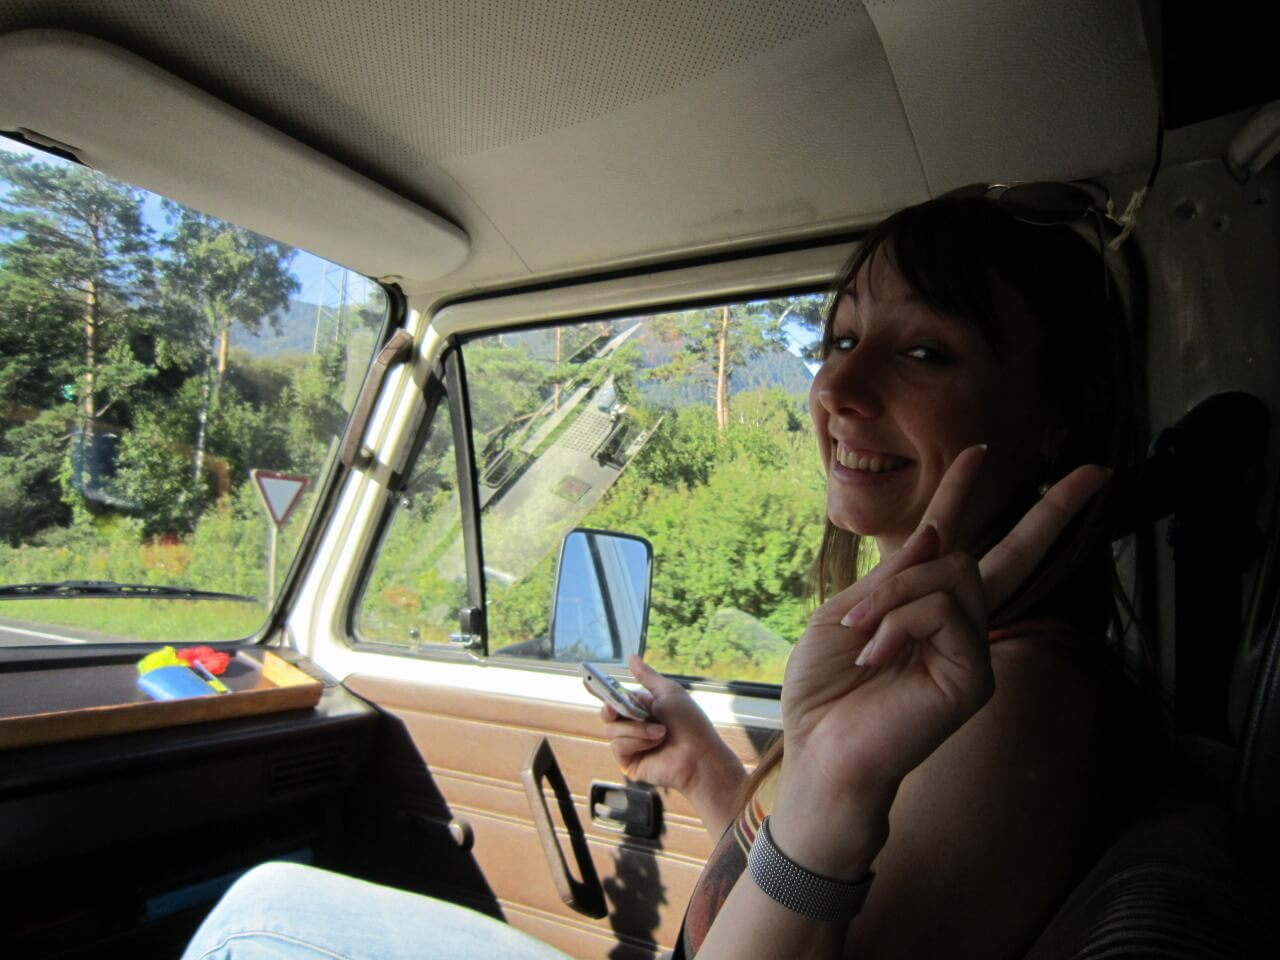
\includegraphics[width=0.4\textwidth, height=5cm, keepaspectratio]{../Bilder/Locarno/3.jpg}
    \caption{Ab in den S�den}
  \end{centering}
\end{wrapfigure} 

Nach einer viel zu kurzen Nacht hiess es um kurz nach 5 Uhr ab auf die F�sse.
Mir fiel es nicht gerade schwer aufzustehen, da mein Magen das klare Kommando zum entleeren seiner selbst gegeben hat.
Ich bekam die volle Wucht des gef�rchteten Nachbrandes nach dem Genuss von scharfem Essen zu sp�ren.
Nach kurzer Zeit war es relativ ruhig im Bus und alle Beifahrer schlummerten und tr�umten von Sonne, Strand und Jack Johnson.
Kaum auf die Westumfahrung aufgefahren, machte uns eine grosse Tafel darauf aufmerksam,
unsere geplante Route durch den Gotthard zu verlassen und dem San Bernadino einen Besuch abzustatten.
Nach kurzer Recherche konnte uns das Argument von fast zwei Stunden Wartezeit �berzeugen und so ging es Richtung Chur dem San Bernadino entgegen.
Der obligate Halt im Heidiland verbrachten wir mit Diskussionen �ber die WC- Bons und nat�rlich kam gerade vor uns ein Car mit einer ganzen Ladung Blumenkohl an, welche erbarmungslos alle verf�gbaren Kassen verstopften.
W�hrend der weiteren Fahrt gen
S�den verpasste Chantal so ziemlich alle sch�nen Sujet beim Studium der Bedienungsanleitung ihrer neuen Kamera.
Die Ersatzbank war eh schon l�nger am d�sen und nickte im Takt der Fahrbahnunebenheiten.
Im gelobten Tessin angekommen, forderte uns das Navi mit einer Strasse von 1.5 Fahrbahnbreiten heraus.
Schon bald kamen wir dann auf dem Camping Delta an.
Die zuerst unfreundliche Dame am Schalter bestand darauf, dass ich ihr pers�nlich meinen Ausweis unter ihre Nase halte.
Als Michel und ich vor ihrem H�uschen auftauchten, verbesserte sich ihre Laune schlagartig.
Der Platz war schnell gefunden und unsere zwei Untermieter machten sich sofort daran ihr neues Zuhause aufzustellen.
Kaum stand das mobile Heim war auch schon der Teufel los und es regnete wie es nur im Tessin seichen kann.
Gl�cklicherweise besserte sich das Wetter wieder und der kleinen Ausfahrt ins Maggia Tal stand nichts mehr im Weg.
Je weiter wir dem Tal folgten, desto schlechter wurde das Wetter.
So fanden wir uns bald
darauf wieder auf dem Weg zur�ck nach Locarno Richtung besseres Wetter.
Ein lauschiges Pl�tzchen an der Maggia war auch schnell gefunden.
Michel und ich unternahmen eine ausgedehnte Erkundungstour und h�pften gazellenartig geschickt von Stein zu Stein um dem kalten Wasser zu entkommen.
Dank eines netten Nachbarn entstand ein Gruppenfoto.
Es wird gemunkelt, dass gewisse Personen nach diesem Foto ihren Psychologen aufsuchen m�ssen um die schrecklichen Bilder aus ihrem Kopf zu verbannen.
Der nette Fotograf parkte sein nur durch feine, hautenge Badehosen bedecktes Geh�nge kniend auf einem Stein vor uns, um einen sicheren \glqq Stand\grqq{} f�r die Kameraausl�sung zu haben.
Die nachfolgende Shoppingtour im Coop geh�rt in das Kapitel: Geh nie mit Hunger einkaufen.
Der Besuch des angrenzenden Bistros konnte man getrost auf die selbe Ebene wie ein Besuch des Bahnhof Buvette am Samstag Morgen stellen.
Lauter merkw�rdige Gestalten mit teils argen modischen Missgeschicken bev�lkerten diesen Ort.
Zur�ck auf dem Campingplatz steigerten wir uns nach einer kurzen Verschnaufpause w�hrend dem Ap�ro in einen wahren Speedmington Rausch.
Da die Flasche Prossecco durchaus Anklang bei der weiblichen Begleitung fand, stieg auch der L�rmpegel und schon bald war dir Umgebung Menschenleer.
Nach einem l�ngeren Ballwechsel war es an der Zeit sich im See abzuk�hlen.
Hart wie M�nner sind, konnten uns auch die vorbeitreibenden Eisberge nicht erschrecken und wir tauchten gen�sslich im Lago.
Fabienne kr�nte das Nachtessen mit ihrer pers�nlichen Interpretation einer Rahmsauce.
Das Bier verschwand schneller als es aus der K�hlbox getragen werde konnte und so begruben wir schon bald die Idee noch nach Locarno zu \glqq wandern\grqq{}.
Das Bett war zu diesem Zeitpunkt eine viel zu gute Alternative.

\begin{figure}[H]
   \centering
      %\sDas Keyboard 4 Professional	ubfloat[CAPTION]{BILDERCODE}\qquad
   \subfloat{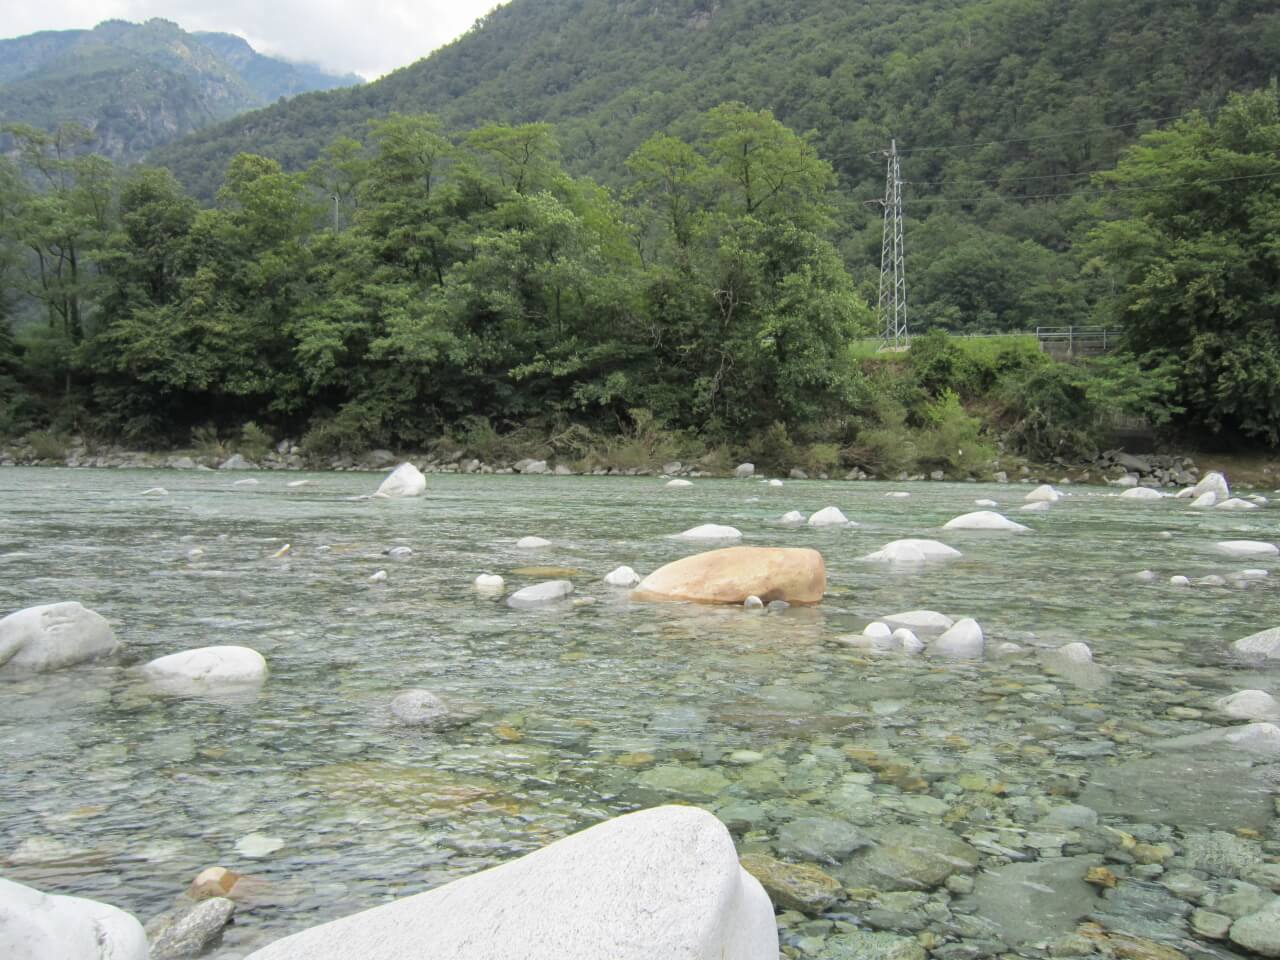
\includegraphics [width=0.3\textwidth]{../Bilder/Locarno/9.jpg}}\quad
   \subfloat{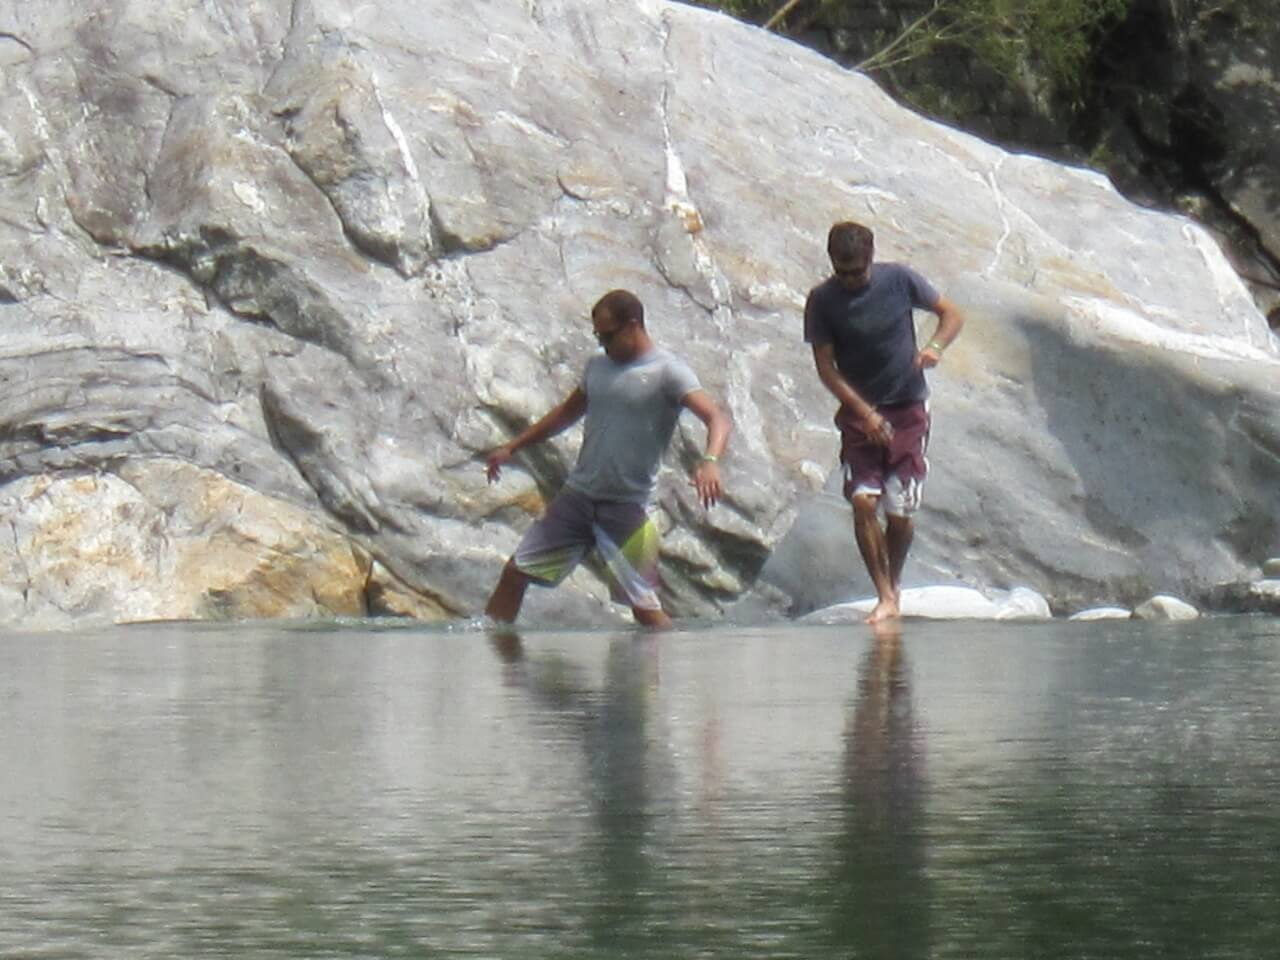
\includegraphics [width=0.3\textwidth]{../Bilder/Locarno/11.jpg}}\quad
   \subfloat{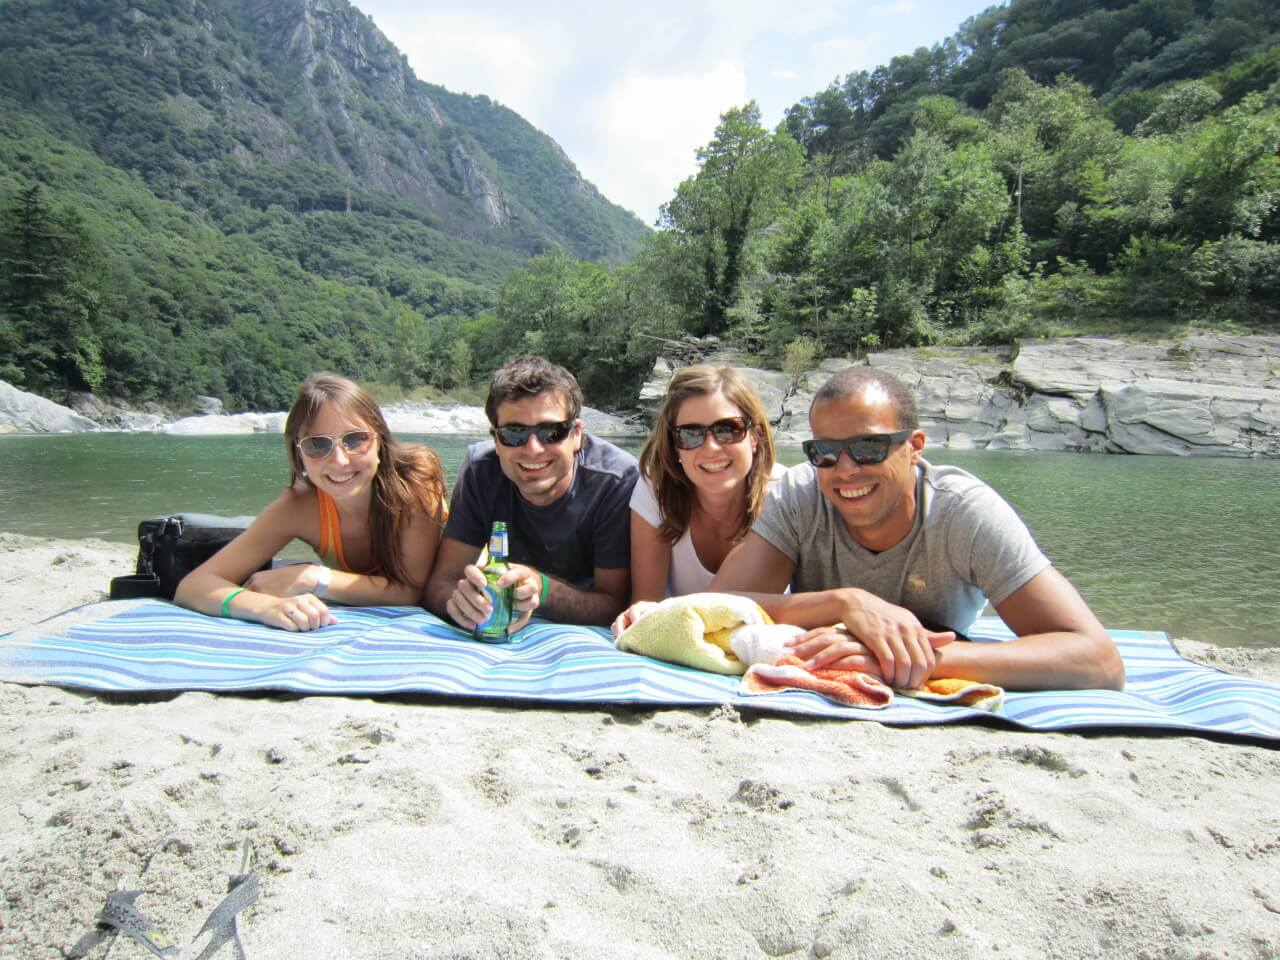
\includegraphics [width=0.3\textwidth]{../Bilder/Locarno/15.jpg}}\quad
   \caption[Action an der Maggia]{Action an der Maggia}
\end{figure}

\subsection{Sonntag 17.07.2011}
Das einheitliche Grau vor dem Fenster liess nichts Gutes erahnen.
Schon w�hrend der Nacht wurde alles mit reichlich Wasser begossen.
Irgendwie gelang es uns trotz allem das Fr�hst�ck im freien w�hrend einer Regenpause zu uns zu nehmen.
Nat�rlich wuchs der Wunsch nach Cannobio an den ber�hmt ber�chtigten Markt zu gehen.
Die Variante mit dem Schiff in das angrenzende Ausland zu fahren wurde nicht gerade positiv aufgenommen.
W�hrend der kurzen Fahrt �ffnete der Himmel alle Schleusen und die Fahrt glich eher einer Bootsfahrt, welche ja kurz vorher noch eher negativ bewertet wurde.
Die Kolonne welche uns Eingangs Cannobio erwartete verhiess nicht Gutes.
Der lokale Sportplatz wird am Sonntag regelm�ssig zum Parkplatz umgebaut und auch wir stellten den Bus in Mitten von anderen Schweizer Schn�ppchenj�ger ab.
Zuerst mussten Moneten organisiert werden.
Die Situation �hnelte sehr stark dem Parkplatzproblem.
Die Nachfrage �bertraf das Angebot.
W�hrend dem Anstehen bekamen wir aus dem fernen Aargau den Hinweis, dass der Markt nur bis um 13:00 Uhr ge�ffnet hat.
Es war jedoch schon nach 12:00 Uhr und diese Tatsache erh�hte den Ausstoss von Stresshormonen beim weiblichen Teil der Gruppe schlagartig.
Das Ziel der Mannschaft war der Teil des Marktes welcher Essbar ist.
W�hrend dieser Zeit stieg das Wasser auf den Strassen auf bis zu 10 cm an und die mit Schirmen bewaffneten Besucher verhakten sich bei jeder engeren Stelle des Marktes und produzierten so Staus, die sich nicht hinter dem bekannten Osterstau vor dem Gotthard verstecken musste.
Einen Platz in einem Restaurant zu finden, nachdem die Marktfahrer begonnen haben ihre St�nde abzubauen stellte sich als n�chste Herausforderung heraus.
Nach kurzem Warten, welches wir mit einem Apero verk�rzten fanden wir vier der begehrten Pl�tze und konnten gen�sslich an der wohlverdienten Pizza knabbern.
Der Weg zur�ck nach Locarno war von einem Element gepr�gt: Wasser.
Genauso wie das Wasser stieg, machten wir uns auch zusehends Sorgen �ber das Zelt auf dem Zeltplatz.
Dort angekommen bot sich uns ein trauriges Bild.
Es hat sich bereits ein massiver See um das Zelt aufgestaut.
Wir blieben zu viert im Bus und verk�rzten uns die feuchte Zeit bis zum Konzert mit einem T�ggeliturnier.
Danach  mussten wir uns m�glichst Wasserdicht verpacken und auf den Weg nach Locarno machen.
Chantal und Fabienne schlugen ein Tempo an, dem wir unm�glich folgen konnten.
Die beiden watschelten wie die Feuerwehr Richtung Konzert.
Chantal schmuggelte gekonnt ihren Knirps in das Konzertgel�nde und auch der Wettergott hatte etwas erbarmen und schloss die Schleusen f�r die n�chste Zeit.
Auf der B�hne spielten bereits the wailers und wir versuchten uns m�glichst geschickt zu positionieren.
Es misslang uns jedoch geh�rig.
Das Publikum war bunt gemischt und wir brachten es fertig uns direkt vor eine Gruppe besoffener Ostschweizer zu stellen.
Trotzdem war das darauf folgende Konzert ein voller Erfolg und auch das Wetter hielt.
Auf dem R�ckweg musste Michel dem irrsinnigen Flip-Flop Marschtempo Tribut zollen.
Sein Knie spielte nicht mehr mit.
Bald schon schliefen wir nach der Ankunft auf dem Campingplatz ein.

\begin{figure}[H]
    \centering
    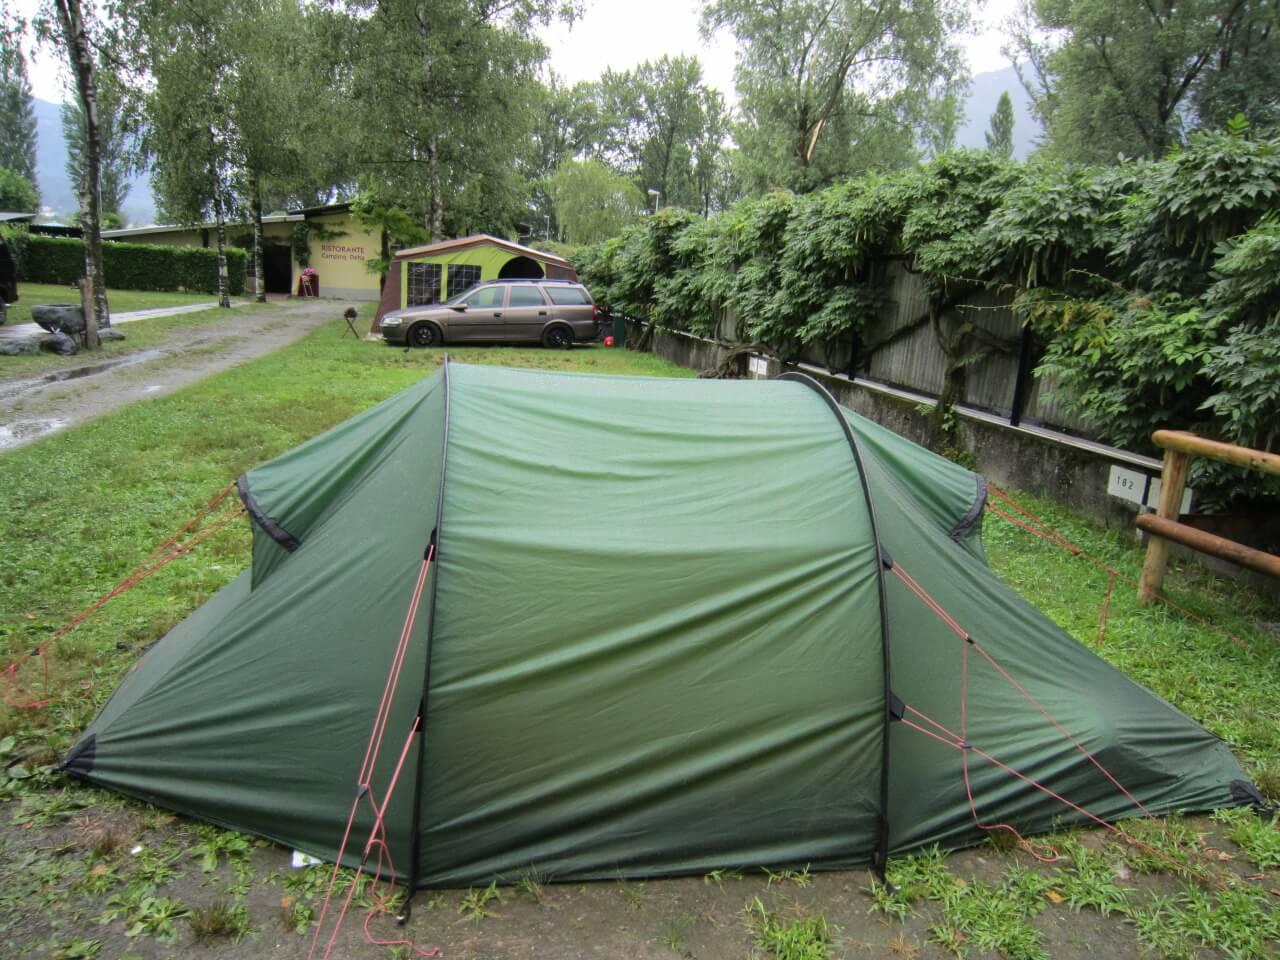
\includegraphics[width=0.6\textwidth]{../Bilder/Locarno/5.jpg}
    \caption{Wasserzelt}
    \label{img:MoonandStars}
\end{figure}

\subsection{Montag 18.07.2011}
Die Sonne blinzelt durch die neuen Vorh�nge.
So erwacht man gerne.
Eine kurze doch eher k�hle Dusche und schon wurde alles f�r das Fr�hst�ck bereit gemacht.
Nach l�ngerer Suche des Siebes f�r die Bialleti konnten wir auch einen Kaffee dazu geniessen und die Sonne trocknete das arg gebeutelte Material.
Doch schon wieder waren dunkle Wolken auf dem Weg zu uns.
So beschlossen wir m�glichst viel einzupacken und uns dann auf den Weg zur�ck ins Mittelland zu machen.
Die R�ckreise verlief absolut problemlos und die R�ckbank war ein weiteres Mal mit schnarchen besch�ftigt.
Da wir sowieso �ber Z�rich fuhren konnten wir Michel gerade noch an der Haust�re abliefern und ich konnte noch kurz beim Eglin vorbeischauen um fehlendes Elektromaterial zu besorgen.
Nach der Reinigung des Busses hiess es schon wieder sich auf die Socken nach Stans zu machen, wo am Dienstag der Ernst des Lebens weiterging.
Die kurze Reise ins Tessin und an das Moon \& Stars war ein voller Erfolg und h�tte nur durch besseres Wetter �bertroffen werden k�nnen.
Wer weiss wer n�chstes Jahr in Locarno auftreten wird? ...

\newpage

\begin{figure}[H]
    \centering
    
\includegraphics[width=\textwidth,height=14cm, keepaspectratio]{../Bilder/Logo/Logo_trans.png}
    \label{img:Logo}
\end{figure}
\vfill
    \begin{center}
        {\huge  Weitere Informationen zum Bus und unseren Reisen sind auf der Homepage {\url{www.jackthebus.com}} zu finden}
\end{center}

\end{document}
